\subsection{Game Explorer}

\begin{figure}[h]
	\centering
	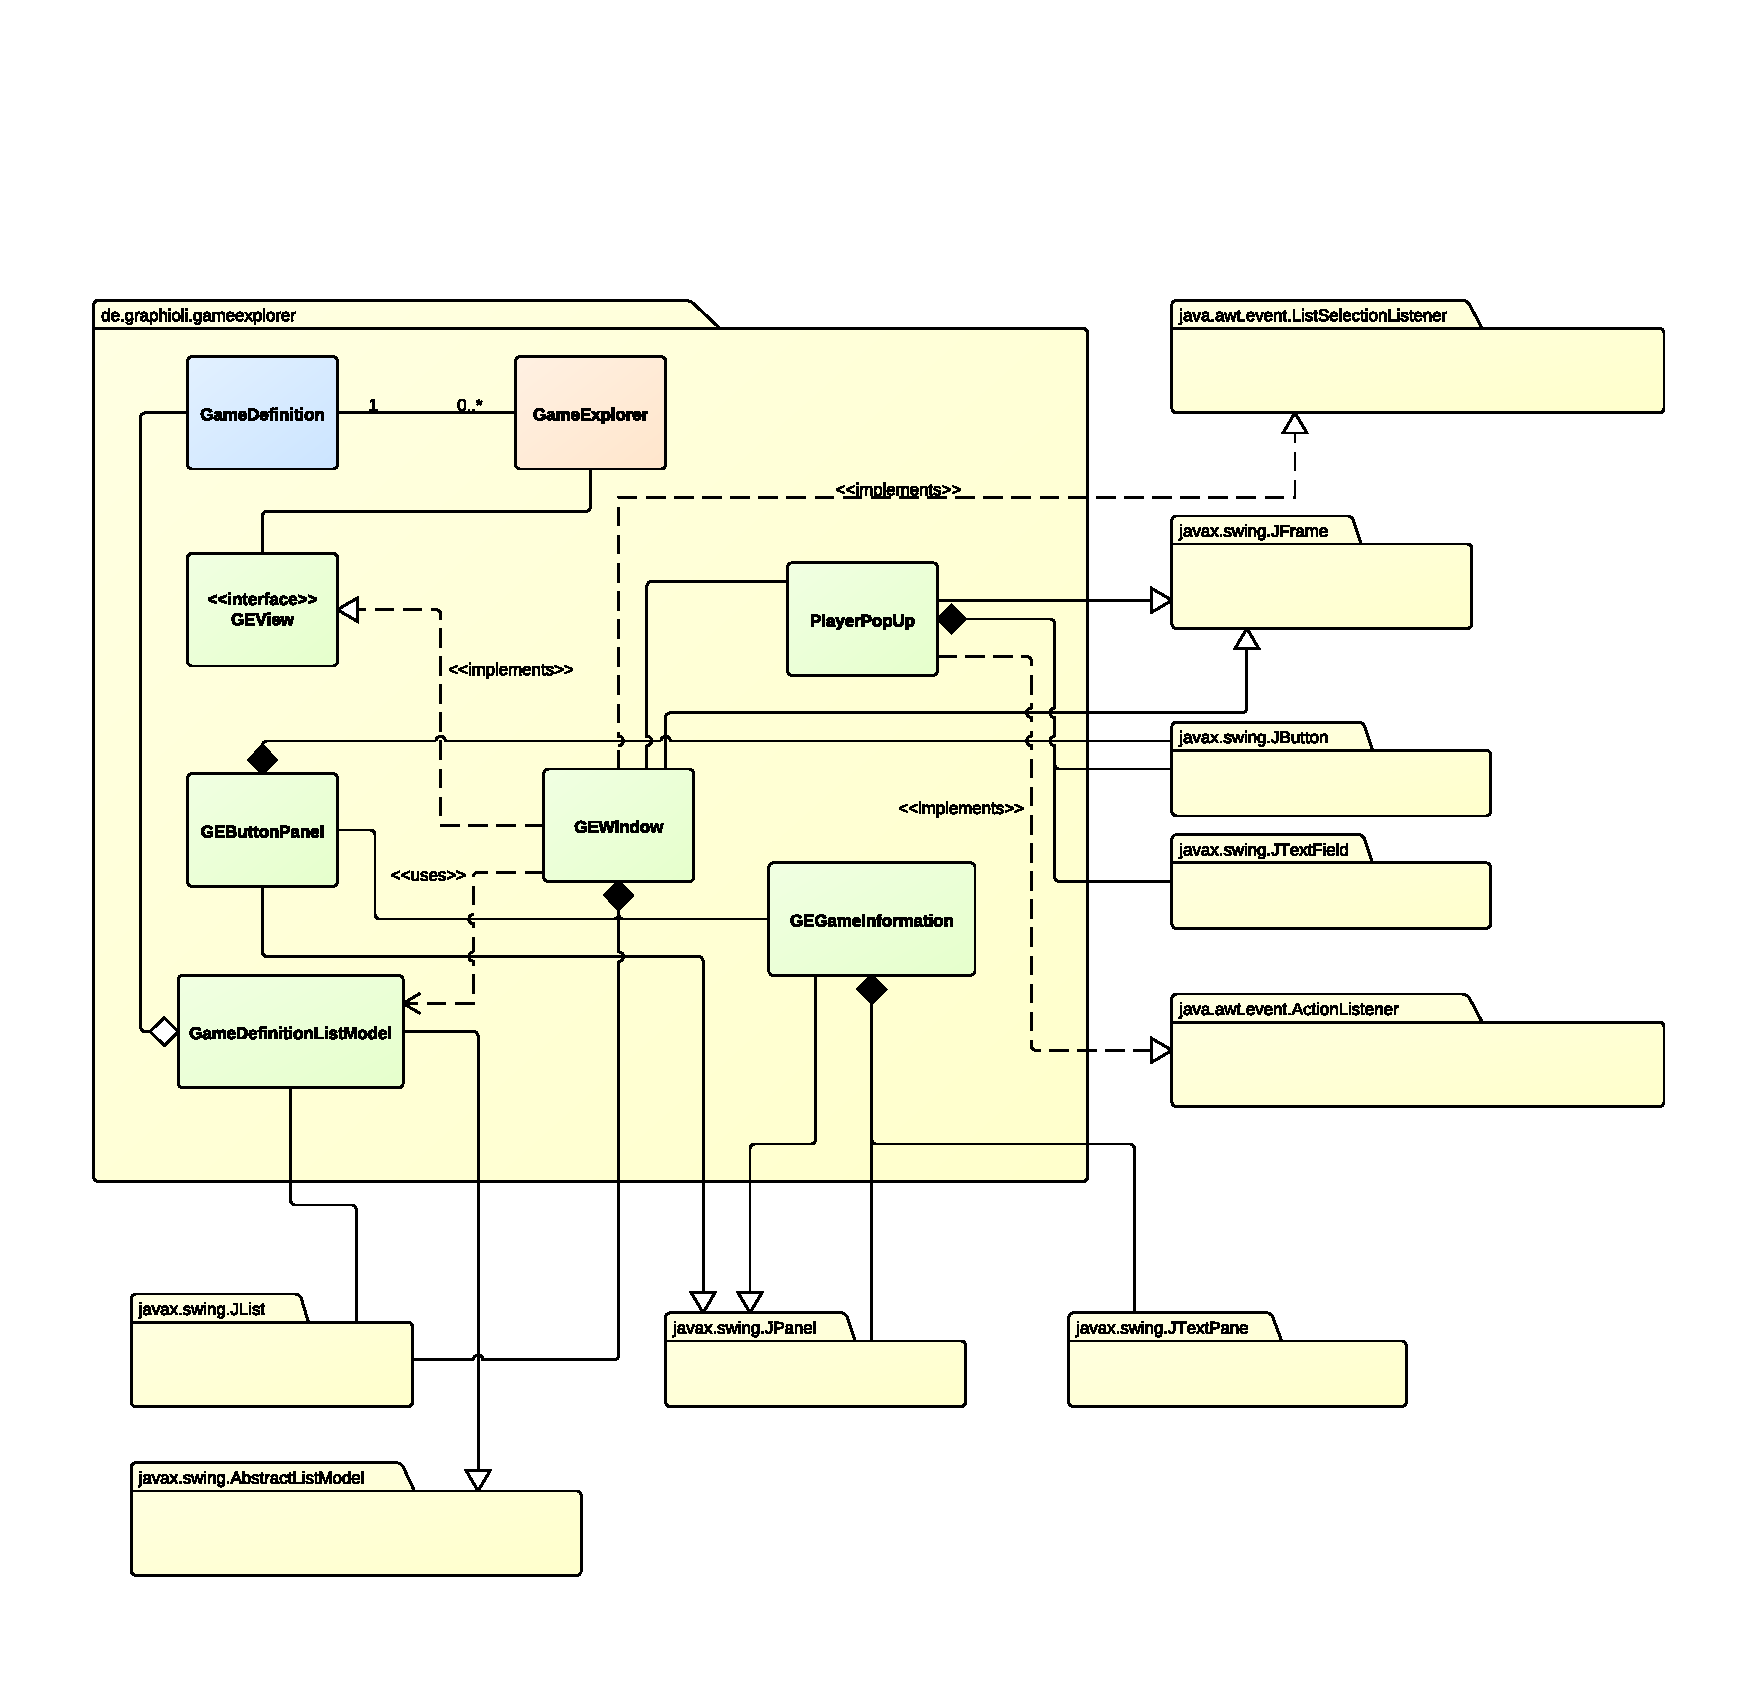
\includegraphics[page=1,width=\textwidth,keepaspectratio]{gameExplorerClassDiagram.pdf}
	\caption{GameExplorer class diagram.}
	\label{img:gameExplorerClassDiagram}
\end{figure}
\pagebreak

% GameExplorer
\class{GameExplorer}{gameexplorer}
The \texttt{GameExplorer} lists the available games and enables the user to select and start one of it.

\centerdash

\paragraph*{Method Summary}
\paragraph*{}
\begin{longtable}{Lp{10cm}}
	\startmethodtable
	\method{public}{GameExplorer(GameManager gameManager)}{ge:gameexplorer} \\
	& Creates a new \texttt{GameExplorer}. \\
	\method{private GameDefinition}{createGameDefinitionFromJSON(String jsonString)}{ge:creategamedefinitionfromjson} \\
	& Parses a \ref{cls:gamedefinition} from a given JSON string. \\
	\method{private Iterable<GameDefinition>}{scanGameFolder()}{ge:scangamefolder} \\
	& Scans the game folder for games and returns the \ref{cls:gamedefinition}s of the games in it. \\
	\method{public boolean}{selectGame(GameDefinition gameDef, Iterable<Player> players)}{ge:selectgame} \\
	& Calls the \ref{cls:gamemanager} to start the game of the given \ref{cls:gamedefinition} and with the given \ref{cls:player}s. \\
	\method{public boolean}{openHelpFile(GameDefinition gameDef)}{ge:openhelpfile} \\
	& Opens the help file of the given \ref{cls:gamedefinition}. \\
	\method{public Iterable<GameDefinition>}{getGameDefinitions()}{ge:getgamedefinitions} \\
	& Returns the \ref{cls:gamedefinition}s of this \texttt{GameExplorer}. \\
	\method{public GameDefinition}{getGameDefinitionAtIndex(int index)}{ge:getgamedefinitionatindex} \\
	& Returns the \ref{cls:gamedefinition} at the specific \texttt{index}. \\
	\hline
\end{longtable}

\pagebreak

% GameDefinition
\class{GameDefinition}{gamedefinition}
This class represents the game's definition, containing crucial information that is needed to start a game.

\centerdash
\paragraph*{Method Summary}
\paragraph*{}
\begin{longtable}{Lp{10cm}}
	\startmethodtable
	\method{public}{GameDefinition({params})}{gd:gamedefinition} \\
	& Creates a new \texttt{GameDefinition} with the specified parameters. \\
	\method{public String}{getName()}{gd:getname} \\
	& Returns the \texttt{name} of this \texttt{GameDefinition}, which is the name of the game. \\
	\method{public int}{getMaxPlayerCount()}{gd:getmaxplayercount} \\
	& Returns the maximum number of players for this specific game. \\
	\method{public int}{getMinPlayerCount()}{gd:getminplayercount} \\
	& Returns the minimum number of players for this specific game. \\
	\method{public String}{getGamePath()}{gd:getgamepath} \\
	& Returns the \texttt{path} of this specific game. \\
	\method{public String}{getDescription()}{gd:getdescription} \\
	& Returns the \texttt{description} of this specific game. \\
	\method{public String}{getFullyQualifiedClassName()}{gd:getfullyqualifiedclassname} \\
	& Returns the fully qualified class name (e.g. ``de.graphioli.game.GraphColoring'') of this specific game. \\
	\method{public BufferedImage}{getScreenshot()}{gd:getscreenshot} \\
	& Returns a \texttt{BufferedImage} that is this game's screenshot. \\
	\method{public File}{getLocalizedString()}{gd:getlocalizedstring} \\
	& Returns a \texttt{String} telling which language file should be used. \\
	\method{public URI}{getHelpFile()}{gd:gethelpfile} \\
	& Returns the \texttt{URI} that links to the help file of this game. \\
	\method{public Iterable<MenuItem>}{getMenu()}{gd:getmenu} \\
	& Returns an iterable list of \texttt{MenuItem}s that will be used to generate this game's custom \texttt{MenuBar}. \\
	\method{public int}{getHorizontalGridPointCount()}{gd:gethorizontalgridpointcount} \\
	& Returns the number of horizontal \ref{cls:gridpoint}s for this specific game. \\
	\method{public int}{getVerticalGridPointCount()}{gd:getverticalgridpointcount} \\
	& Returns the number of vertical \ref{cls:gridpoint}s for this specific game. \\
	\method{public boolean}{isDirectedGraph()}{gd:isdirectedgraph} \\
	& Returns whether the game's graph is directed. \\
	\hline
\end{longtable}

\pagebreak

% GameExplorerView (interface)
\interface{GEView}{geview}
This interface defines the methods the \ref{cls:gameexplorer} uses to communicate with its \gls{GUI}. \\

\centerdash

\paragraph*{Method Summary}
\paragraph*{}
\begin{longtable}{Lp{10cm}}
	\startmethodtable
	\method{public boolean}{registerController(GameExplorer gameExplorer)}{gev:registercontroller} \\
	& Registers the controller for the \ref{cls:gameexplorer} user interface. \\
	\method{public boolean}{generateView()}{gev:generateview} \\
	& Generates the user interface of the \ref{cls:gameexplorer}. \\
	\hline
\end{longtable}

\pagebreak

% GameExplorerWindow
\class{GEWindow}{gewindow}
\createindentedlist{java.lang.Object, java.awt.Component, java.awt.Container, java.awt.Window, java.awt.Frame, javax.swing.JFrame, de.graphioli.gameexplorer.GEWindow}
This class represents the main window of the \ref{cls:gameexplorer}. \\

\begin{description}
	\item[All Implemented Interfaces] \hfill \\
	\ref{cls:geview}, java.awt.event.ListSelectionListener
\end{description}

\centerdash

\paragraph*{Method Summary}
\paragraph*{}
\begin{longtable}{Lp{10cm}}
	\startmethodtable
	\method{public boolean}{generateView()}{gew:generateview} \\
	& Generates the graphical user interface of the \ref{cls:gameexplorer} (\ref{cls:gegameinformation}, \ref{cls:gebuttonpanel} and \texttt{JList} containing the \ref{cls:gamedefinitionlistmodel}). \\
	\method{public void}{valueChanged(ListSelectionEvent event)}{gew:valuechanged} \\
	& Called by the \texttt{JList} when its selection has changed to update the remaining graphical elements of this \texttt{GEWindow}. \\
	\method{public boolean}{openHelpFile()}{gew:openhelpfile} \\
	& Calls \ref{ge:openhelpfile} of \ref{cls:gameexplorer} with the \texttt{selectedGameDefinition}. \\
	\method{public boolean}{openPlayerPopUp()}{gew:openplayerpopup} \\
	& Creates and shows a \ref{cls:playerpopup} for \ref{cls:player} selection. \\
	\method{public boolean}{onPlayerPopUpReturn(Iterable<Player> players)}{gew:onplayerpopupreturn} \\
	& Called by the \ref{cls:playerpopup} when it has finished and triggers the start of the game. \\
	\hline
\end{longtable}

\pagebreak

% PlayerPopUp
\class{PlayerPopUp}{playerpopup}
\createindentedlist{java.lang.Object, java.awt.Component, java.awt.Container, java.awt.Window, java.awt.Frame, javax.swing.JFrame, de.graphioli.gameexplorer.PlayerPopUp}

Represents a pop-up window that is used to select the the number of players and their names for a game. \\
\begin{description}
	\item[All Implemented Interfaces] \hfill \\
	java.awt.event.ActionListener
\end{description}

\centerdash

\paragraph*{Method Summary}
\paragraph*{}
\begin{longtable}{Lp{10cm}}
	\startmethodtable
	\method{public}{PlayerPopUp(int minPlayer, int maxPlayer)}{ppu:playerpopup} \\
	& Creates a \texttt{PlayerPopUp}. \\
	\method{public void}{actionPerformed(ActionEvent event)}{ppu:gamedefinitionlistmodel} \\
	& Callback method for the \texttt{JButtons}, that creates the \ref{cls:player}s based on the input and calls \ref{gew:onplayerpopupreturn}. \\
	\hline
\end{longtable}

\pagebreak

% GameDefinitionListModel
\class{GameDefinitionListModel}{gamedefinitionlistmodel}
Represents a data model that provides the \texttt{JList} with its content. \\

\centerdash

\paragraph*{Method Summary}
\paragraph*{}
\begin{longtable}{Lp{10cm}}
	\startmethodtable
	\method{public}{GameDefinitionListModel(Iterable<GameDefinition> definitions)}{gdlm:gamedefinitionlistmodel} \\
	& Creates a new \texttt{GameDefinitionListModel} with the given \ref{cls:gamedefinition}s. \\
	\method{public Object}{getElementAt(int index)}{gdlm:getgamedefinitionatindex} \\
	& Returns the \texttt{name} of the \ref{cls:gamedefinition} at the given \texttt{index} so the \texttt{JList} can display it. \\
	\hline
\end{longtable}

\pagebreak

% GameExplorerGameInformation
\class{GEGameInformation}{gegameinformation}
\createindentedlist{java.lang.Object, java.awt.Component, java.awt.Container, javax.swing.JComponent, javax.swing.JPanel, de.graphioli.gameexplorer.GEGameInformation}

Organizes the output of the screenshot and the description of the game. \\

\centerdash

\paragraph*{Method Summary}
\paragraph*{}
\begin{longtable}{Lp{10cm}}
	\startmethodtable
	\method{public boolean}{setDescription(String description)}{gegi:setdescription} \\
	& Sets the \texttt{description} of the game and updates the display. \\
	\method{public boolean}{setScreenshot(BufferedImage screenshot)}{gegi:setscreenshot} \\
	& Sets the \texttt{screenshot} of the game and updates the display. \\
	\hline
\end{longtable}

\pagebreak

% GameExplorerButtonPanel
\class{GEButtonPanel}{gebuttonpanel}
\createindentedlist{java.lang.Object, java.awt.Component, java.awt.Container, javax.swing.JComponent, javax.swing.JPanel, de.graphioli.gameexplorer.GEButtonPanel}

Organizes \texttt{JButtons} and listens to them calling the specific methods in the \ref{cls:gewindow}. \\
\begin{description}
	\item[All Implemented Interfaces] \hfill \\
	java.awt.event.ActionListener
\end{description}

\centerdash

\paragraph*{Method Summary}
\paragraph*{}
\begin{longtable}{Lp{10cm}}
	\startmethodtable
	\method{public boolean}{setButtonsActive(boolean isActive)}{gebp:setbuttonsactive} \\
	& Sets the \texttt{JButtons} (in)active. \\
	\method{public boolean}{actionPerformed(ActionEvent event)}{gebp:actionperformed} \\
	& Invoked if a \texttt{JButton} is clicked and calls the specific methods in the \ref{cls:gewindow}. \\
	\hline
\end{longtable}
